\section{Gabriel Deployment System}

Previous research on wearable cognitive assistance~\cite{chen2017empirical} has
focused on meeting application latency requirements and assumed abundant
resources on the cloudlets. However, when there are many users in the system
and the utilizations of system resources are high, both the compute and the
memory at the cloudlets can become scarce. Reduction of the application
footprint on cloudlets is needed in order to scale better.

\begin{figure}[h]
  \centering
  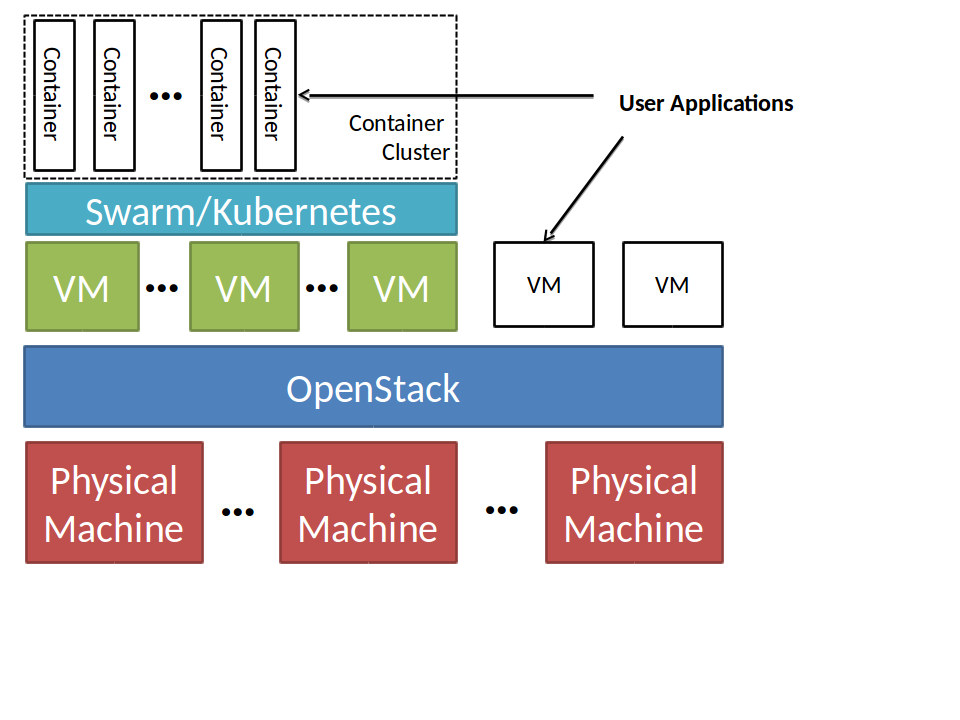
\includegraphics[trim={0 1.5in 0 0},clip,width=5in]{FIGS/cloudlet-gateway}
  \caption{Container and Virtual Machine Virtualization on Cloudlets}
  \label{fig:cloudlet-gateway}
  \end{figure}

Virtual machines (VMs) have been used to provide isolation among edge node
tenants~\cite{ha2014towards}. While VMs virtualize at the hardware level and
provide strong isolation among tenants, they also have a large footprint since
each virtual machine has its own kernel. In the meantime, some applications do
not need the strong isolation provided by VMs. For example, applications
published by the same developer or company would have stronger trusts about the
integrity of the software. Therefore, for these applications, using more
lightweight virtualization constructs, for instance, containers, can help reduce
the application footprint on cloudlets.

Figure~\ref{fig:cloudlet-gateway} shows an edge node implementation that
combines lightweight container virtualization with strongly isolated virtual
machines. It adopts a Container-on-top-of-VM approach. Application providers on
the cloudlets can create container clusters for managing multiple applications
or instances of an application using the lightweight containers. In the
meantime, different providers are isolated by VMs for better control. The edge
node deployment system also supports applications to use a combination of
virtual machines and containers. For example, an application might have some
components in Windows VMs while other components run inside Linux containers.
When this combination of virtualization is used, the system provides a DNS
service to help resolve hostnames.

\begin{figure}[h]
  \centering
  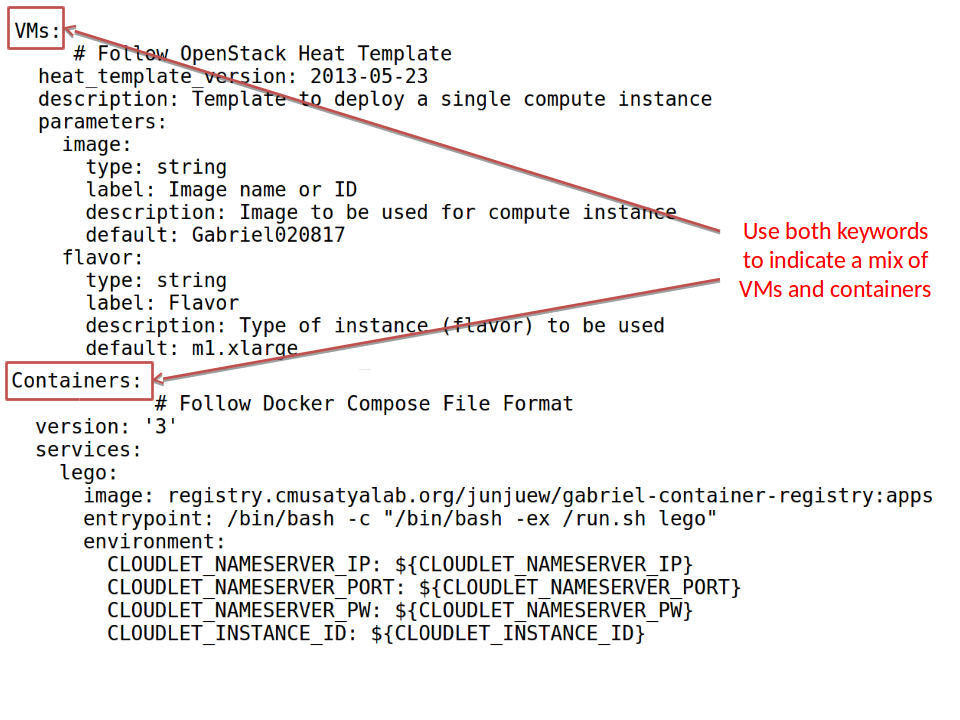
\includegraphics[trim={0 1.5in 0 0},clip,width=5in]{FIGS/cloudlet-app-configuration}
  \caption{Application Deployment Template with Virtualization Type Specified}
  \label{fig:cloudlet-app-configuration}
  \end{figure}


In order to specify virtualization techniques to use, developers only need to
modify their existing orchestration templates to include their choice of
virtualization. The system's annotation uses YAML~\cite{ben2005yaml} and follows
the convention of orchestration frameworks, including OpenStack Heat and Docker
Swarm. Figure~\ref{fig:cloudlet-app-configuration} shows an application
configuration file that adopts a mixed of virtual machine and container
virtualization. Components with different virtualization are separated into
different sections. Developers mark each section with the virtualization
technique they want to use. Specifications inside each section correspond to the
template consumed by the underlying orchestration frameworks.
